\documentclass[tikz,border=10pt]{standalone}
\usepackage{tikz}
\begin{document}
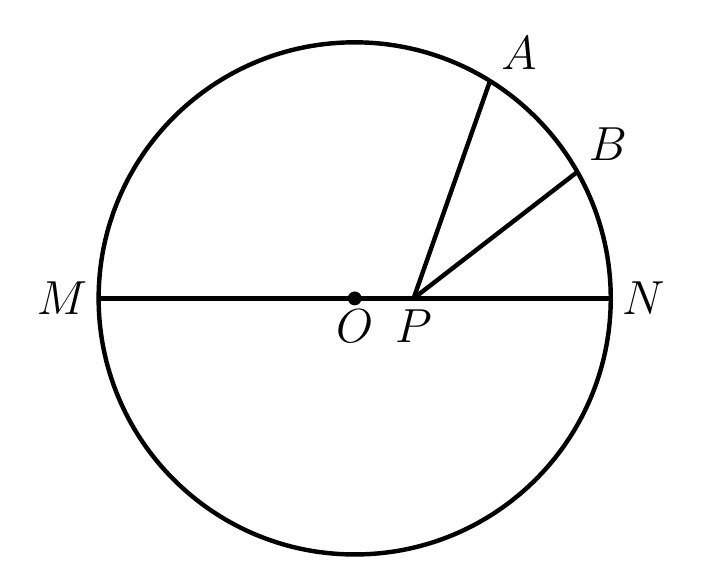
\begin{tikzpicture}[line join=round, line width=1.6pt]
  % Scale s = 0.020672 cm/px, origin at O (px 233.27, 201.1)
  \coordinate (O) at (0,0);
  \coordinate (M) at (-3.252,0);
  \coordinate (N) at (3.252,0);
  \coordinate (P) at (0.748,0);
  % A exactly on the circle (radius 3.252 cm, angle 58.1 deg)
  \coordinate (A) at (58.1:3.252);
  % B exactly on the circle (radius 3.252 cm, angle 29.6 deg)
  \coordinate (B) at (29.6:3.252);

  % Circle and diameter MN
  \draw (O) circle (3.252);
  \draw (M) -- (N);

  % Segments PA and trimmed PB (ends on circle)
  \draw (P) -- (A);
  \draw (P) -- (B);

  % Centre dot (enlarged)
  \fill (O) circle (2.5pt);

  % Labels
  \node[left] at (M) {\fontsize{16.5}{19.8}\selectfont $M$};
  \node[right] at (N) {\fontsize{16.5}{19.8}\selectfont $N$};
  % O label centred directly below the centre point
  \node[below] at (O) {\fontsize{16.5}{19.8}\selectfont $O$};
  \node[below] at (P) {\fontsize{16.5}{19.8}\selectfont $P$};
  % A label up and slightly right of its endpoint
  \node[anchor=south west] at (A) {\fontsize{16.5}{19.8}\selectfont $A$};
  \node[above right] at (B) {\fontsize{16.5}{19.8}\selectfont $B$};
\end{tikzpicture}
\end{document}